%!TEX program = xelatex
%% Copyright (C) 2025 傅祉珏 杨程骏 谢敬豪
%% 
%% 此文件是《Homework4 学业困难学生识别》的LaTeX源码,依据AGPLv3许可证发布。
%% 完整许可证文本见项目根目录LICENSE文件,附加限制条款见ADDITIONAL_TERMS.md。
%% 
%% 禁止商业用途,学术使用需保留本声明。
%% 源码仓库:https://github.com/Billiefu/YatPR

% SPDX-FileCopyrightText: 2025 傅祉珏 杨程骏 谢敬豪
% SPDX-License-Identifier: AGPL-3.0-or-later
% SPDX-Additional-Clauses: see ADDITIONAL_TERMS.md

\documentclass[a4paper, utf8]{ctexart}
\usepackage[scr=boondox,cal=esstix]{mathalpha}
\usepackage[fontset=Fandol]{ctex}
\usepackage{draftwatermark}
\usepackage{algpseudocode}
\usepackage{algorithmicx}
\usepackage{anyfontsize}
\usepackage{indentfirst}
\usepackage{subcaption}
\usepackage{algorithm}
\usepackage{amsfonts}
\usepackage{enumitem}
\usepackage{tabularx}
\usepackage{fancyhdr}
\usepackage{geometry}
\usepackage{graphicx}
\usepackage{abstract}
\usepackage{amsmath}
\usepackage{lipsum}

% 设置页面间距
\geometry{a4paper,left=31mm,right=31mm,top=25mm,bottom=25mm}
% 章节标题左对齐
\CTEXsetup[format={\Large \bfseries}]{section}
% 段首缩进2字符
\setlength{\parindent}{2em}
% 设置页眉及页脚 页码
\pagestyle{fancy}
\fancyhf{}
\fancyhead[C]{}
\fancyhead[L]{模式识别\ \ Homework4}
\fancyhead[R]{算法比较与深度分析实践——学业困难学生识别}
\fancyfoot[C]{\thepage}
\fancyfoot[L,R]{}

% 使宋体可加粗
\setCJKfamilyfont{zhsong}[AutoFakeBold = {2.17}]{SimSun}
\renewcommand*{\songti}{\CJKfamily{zhsong}}

% 定义标题 作者及单位信息
\title{\songti \Large \textbf{Homework4 \ \  学业困难学生识别}}
\author{\fangsong 傅祉珏 \ \  杨程骏 \ \  谢敬豪}
\date{\fangsong 中山大学计算机学院 \ \  广东广州 \ \  510006}

% 版权信息水印
\SetWatermarkText{Copyright\ \copyright\ 2025\ 傅祉珏\ 杨程骏\ 谢敬豪}
\SetWatermarkScale{0.28}
\SetWatermarkAngle{45}
\SetWatermarkColor[gray]{0.8}

\begin{document}

	\begin{titlepage}
		\centering
		\rule{\textwidth}{1pt}
		\vspace{0.02\textheight}
		
		{\LARGE \kaishu 模式识别 \quad SYSU\ CSE\ 2024-2 \quad 课程作业}
		
		\vspace{0.02\textheight}
		
		{\Huge \songti \bfseries Homework4 \  学业困难学生识别}
		
		\vspace{0.025\textheight}
		\rule{0.83\textwidth}{0.4pt}
		\vspace{0.05\textheight} 
		\begin{figure}[htbp]
			\centering
			
\includegraphics[width=8cm, height=8cm]{./figure/计院院徽.jpg}
		\end{figure}
		
		\vspace{0.04\textheight} 
		{\Large 课程编号:\textsc{DCS299}}
		
		\vspace{0.025\textheight} 
        {\Large 组长信息:\textsc{傅祉珏\ 21307210}}

        \vspace{0.025\textheight} 
        {\Large 组员1信息:\textsc{杨程骏\ 22331111}}

        \vspace{0.025\textheight} 
        {\Large 组员2信息:\textsc{谢敬豪\ 22336255}}
		
		\vspace{0.025\textheight} 
		{\Large 项目截止时间:\textsc{2025年7月6日}}
		
		\vspace{0.05\textheight} 
		\vfill
		
		{\large \today}
		\vspace{0.1\textheight}
		\rule{\textwidth}{1pt}
	\end{titlepage}
	\let\cleardoublepage\clearpage
	
	\maketitle
	
	\renewcommand{\abstractname}{\large \textbf{摘要}}
	\begin{abstract}
		本次实验以“学业困难学生识别”为核心任务,围绕教育数据挖掘中的分类问题,系统实现并比较了逻辑斯谛回归、支持向量机(SVM)、决策树、K近邻(KNN)、K-means 聚类、多层感知机(MLP)等六种常见判别算法,并进一步引入基于堆叠策略的集成学习方法,以提升模型的泛化能力与稳定性。实验在真实学生成绩数据集上开展,评估指标涵盖准确率、损失函数值、训练时间以及类别分布等。结果表明,不同算法在处理学生学业表现识别问题时存在显著差异,其中 MLP 与集成模型在整体性能上具有更优表现,K-means 等无监督方法在集成后亦表现出较强的协同潜力。本实验为构建高效可靠的学业预警系统提供了方法参考,也为教育数据智能分析的深入研究提供了实践依据。
		
		\noindent{\textbf{\heiti 关键词:}学业困难识别;教育数据挖掘;分类算法;集成学习;模型比较。}
	\end{abstract}
	
	\section{引言}
	
	在大规模在线学习平台迅速普及的背景下,如何及时发现可能面临学业困难的学生,已成为教育技术领域的重要课题\cite{ref5,ref18,ref20}。一方面,在线教育平台积累了大量可用于行为分析的数据,如视频学习时长、论坛活跃度、测验成绩、登录频率等,这些数据反映了学生的学习状态与行为特征\cite{ref14,ref15}。另一方面,学生的学习过程具有高度个体差异性,仅凭表面行为难以直观判断其学业风险。因此,借助机器学习算法对早期行为数据进行建模与分析,成为预测学生学习结果、提前干预的重要手段\cite{ref13,ref19,ref24}。
	
	本实验聚焦于\textbf{\songti “学业困难学生识别”}问题,基于开放大学学习分析数据集(OULAD),选取学生在某门课程前四周的匿名行为数据,包括课程视频观看时长、测验尝试次数、论坛互动频率、登录习惯等特征,构建并对比多种分类模型的性能。在对问题建模的过程中,我们尝试了多种具有代表性的算法,包括线性分类器、决策树、支持向量机、多层感知机等,分别代表不同类型的学习方法,以探索各类模型在此类行为数据下的表现优势与局限\cite{ref3,ref7,ref10,ref23}。
	
	特别地,为进一步提升预测准确率与模型鲁棒性,我们还引入了\textbf{\songti 集成学习}策略,探究多模型融合是否能有效结合不同模型在特征学习上的互补性\cite{ref6,ref9,ref25}。通过对比融合模型与单一模型的性能差异,我们希望回答一个关键问题:在教育行为数据稀疏、噪声较大的背景下,模型集成是否是提升预测性能的可行方案\cite{ref16,ref26}。
	
	本实验不仅关注模型的最终准确度,还从训练效率、超参数敏感性、特征依赖、可解释性与模型复杂度等多维度展开深入分析。通过全面的实验设计与结果对比,我们旨在促进对模式识别方法在教育预测任务中的理解,提升模型分析与实证研究的能力,同时也为教育干预实践提供数据支持与决策参考。
	
	\section{相关工作}
	
	在近年来教育数据挖掘(Educational Data Mining, EDM)与学习分析(Learning Analytics, LA)研究中,基于行为数据识别学业困难学生已成为关注热点\cite{ref5,ref18,ref20}。相关研究主要聚焦于通过对在线学习平台上学生的早期互动行为建模,以预测其后续学业表现,从而实现及时预警与干预\cite{ref14,ref26}。
	
	许多早期工作采用线性分类器(如逻辑回归、感知机)等方法对学生学习状态进行预测\cite{ref13,ref19}。这类方法具有较强的可解释性,能够提供各行为特征对最终结果的权重,便于教师进行教学决策。但在线性不可分场景下,分类性能常常受到限制。为提升模型表现,研究者逐步引入了非线性方法,如支持向量机(SVM)与决策树模型\cite{ref7,ref23}。这些方法能较好捕捉复杂行为与结果之间的非线性关系,尤其适用于特征维度较高但样本量有限的教育数据\cite{ref16}。
	
	近年来,随着深度学习的发展,神经网络模型也被广泛应用于教育预测任务中,尤其在处理多模态行为特征、时间序列建模方面表现出较强能力\cite{ref4,ref11,ref22}。例如,卷积神经网络(CNN)与循环神经网络(RNN)已被用于学生学习轨迹分析与风险识别\cite{ref22}。不过,深度模型虽然在准确率上具有潜力,但其训练成本较高,且可解释性较差,这在教育场景中引发一定争议\cite{ref11}。
	
	为兼顾性能与稳定性,部分研究进一步采用集成学习(Ensemble Learning)方法,将多种模型的预测结果融合,以提升整体泛化能力\cite{ref6,ref9}。如Bagging与Boosting方法被用于学生成绩预测与学习风格分类任务中\cite{ref10,ref16}。此外,Stacking等模型融合策略可以结合不同模型的特长,提高对不平衡数据中少数类(如“困难学生”)的识别鲁棒性\cite{ref12,ref25}。这与本实验所采用的融合方法思路一致,尤其适用于“困难学生”这一小样本、复杂特征的目标群体。
	
	在特征层面,许多研究也表明学生的早期学习行为(如视频观看时间、测验参与度、讨论区活跃度等)对其学习成果具有显著影响\cite{ref14,ref15,ref24}。因此,恰当的特征表示与降维方法(如主成分分析 PCA、判别分析 LDA)也被广泛用于提升模型效率与可解释性\cite{ref3,ref19}。这与课程中“第二章 特征提取与表示”与“第三章 主成分分析”所介绍的内容紧密相关。
	
	综上所述,当前关于学业困难学生识别的研究涵盖了从浅层模型到深度学习、从单模型到集成方法、从原始行为特征到降维表示的多种策略。本实验在此基础上,结合多种分类算法与模型融合机制,在准确性、效率与可解释性之间寻求平衡,并对比各方法在教育行为数据下的适用性与表现差异,进一步拓展上述研究方向的教学实践与实证分析维度。
	
	\section{方法}
	
	\subsection{判别模型}
	
	为识别可能面临学业困难的学生,我们选取了六种在模式识别和教育数据分析中常用的算法,涵盖了线性模型、非线性模型、实例学习方法、聚类方法与神经网络等多个类别。这些模型在处理结构化行为数据和不平衡分类问题上各具优势,适合对比研究其在教育场景下的适用性与性能差异\cite{ref5,ref16,ref19}。
	
	\subsubsection{逻辑斯谛回归}
	
	逻辑斯谛回归是一种广泛应用于分类任务的线性模型。其基本思想是将输入特征的线性组合映射到概率空间,用以估计样本属于某一类别的概率\cite{ref3,ref13,ref26}。在多分类场景下,逻辑回归采用 Softmax 函数对所有类别进行归一化处理。模型参数通过最小化交叉熵损失函数进行学习,训练过程中通常采用梯度下降法,并结合标准化与正则化策略以提升模型稳定性和泛化能力。在二分类问题中,逻辑回归模型形式如下:
	
	\vspace{-.5em}
	\begin{equation}
		P(y=1|\mathbf{x})=\sigma(\mathbf{w}^T\mathbf{x}+b)=\frac{1}{1+\exp(-\mathbf{w}^T-b)}
	\end{equation}
	
	其中,$\sigma(\cdot)$ 是 Sigmoid 函数,$\mathbf{w}$ 和 $b$ 分别为权重向量与偏置项。在多分类场景下,逻辑回归采用 Softmax 函数对所有类别进行归一化处理:
	
	\vspace{-.5em}
	\begin{equation}
		P(y=k|\mathbf{x})=\frac{\exp(\mathbf{w}^T_k\mathbf{x}+b_k)}{\sum^{K}_{j=1}\exp(\mathbf{w}_j^T+\mathbf{x}+b_j)}
	\end{equation}
	
	模型参数通过最小化交叉熵损失函数进行学习,形式为:
	
	\vspace{-.5em}
	\begin{equation}
		\mathcal{L}=-\frac{1}{n}\sum^n_{i=1}\sum^{K}_{k=1}\mathbb{I}(y_i=k)\log P(y_i=k|\mathbf{x}_i)
	\end{equation}
	
	其中,$\mathbb{I}(\cdot)$ 表示指示函数。训练过程中通过梯度下降法对权重和偏置进行优化更新,并可结合学习率衰减策略提升收敛稳定性。在模型实现中,通常需对输入特征进行标准化处理,以加快训练过程并减少数值波动。
	
	\subsubsection{支持向量机}
	
	支持向量机是一种基于间隔最大化原则的判别式分类模型。在线性不可分的情形下,引入核函数映射至高维空间可有效提升模型的非线性拟合能力。在教育数据中,SVM 被广泛用于小样本、高维特征场景的分类任务\cite{ref7,ref19}。此外,结构化多类 SVM 与正则化策略相结合,可进一步提高其在实际任务中的性能表现与鲁棒性。在线性可分的情况下,SVM 试图在样本空间中找到一个能够最大化类别间隔的超平面,其目标函数如下:
	
	\vspace{-.5em}
	\begin{equation}
		\min_{\mathbf{w},b}\frac{1}{2}\left\| \mathbf{w} \right\|^2 \quad \text{s.t.} \quad y_i(\mathbf{w}^T\mathbf{x}_i+b)\geq1,\forall i
	\end{equation}
	
	对于现实中常见的线性不可分情形,可引入松弛变量并通过合适的损失函数进行优化。在多分类任务中,常采用一对多或一对一策略构建多个二分类器。本实验中使用的是结构化多类 SVM,采用如下的损失函数进行训练:
	
	\vspace{-.5em}
	\begin{equation}
		\mathcal{L}=\frac{1}{n}\sum^n_{i=1}\sum_{j\neq y_i}\max(0, \mathbf{w}^T_j\mathbf{x}_i-\mathbf{w}^T_{y_i}\mathbf{x}_i+\Delta)
	\end{equation}
	
	其中 $\Delta$ 表示预设的间隔常数,$\mathbf{w}_j$ 是第 $j$ 类的权重向量。该损失函数鼓励正确类别的得分高于其他类别至少 $\Delta$,从而在特征空间中形成明确的判别边界。模型训练一般采用小批量梯度下降法进行参数更新,并引入 $L_2$ 正则项抑制过拟合:
	
	\vspace{-.5em}
	\begin{equation}
		\mathcal{L}_{\text{reg}}=\mathcal{L}+\lambda \left\|W\right\|^2_2
	\end{equation}
	
	特征输入在训练前通常需要归一化,以防止尺度不一致影响间隔计算。
	
	\subsubsection{决策树}
	
	决策树是一种基于树结构的分类与回归模型,CART(Classification and Regression Tree)是其中一种典型实现。\cite{ref23}其基本思想是在每个节点选择最优特征与划分点,将样本集划分为两个子集,递归地构建子树直至满足停止条件。决策树具有高度可解释性,适用于对教育预测任务中行为特征进行可视化分析与推理建模\cite{ref15,ref16}。CART 模型使用基尼指数(Gini Impurity)作为节点划分的准则,定义如下:
	
	\vspace{-.5em}
	\begin{equation}
		\text{Gini}(S)=1-\sum^K_{k=1}p^2_k
	\end{equation}
	
	其中,$p_k$ 表示当前节点中第 $k$ 类样本的比例。每个候选划分点的增益(Gain)计算为:
	
	\vspace{-.5em}
	\begin{equation}
		\text{Gain}=\text{Gini}(S)-\left( \frac{\left| S_L \right|}{\left| S \right|}\text{Gini}(S_L) + \frac{\left| S_R \right|}{\left| S \right|}\text{Gini}(S_R) \right)
	\end{equation}
	
	其中 $S_L$ 和 $S_R$ 分别为划分后左、右子集,$|S|$ 表示样本数量。模型选择具有最大信息增益的划分方式作为当前节点的分裂标准。
	
	树的生长在以下条件下终止:样本纯度达到要求、当前深度超过设定最大值,或节点样本数小于最小分裂样本数。最终叶节点上的类别通过多数投票方式确定。
	
	CART 模型无需对特征进行线性假设,能够自动建模特征之间的非线性关系,且结构直观,便于可视化和解释。其训练过程为一种贪心算法,不保证全局最优,但能高效完成复杂任务的数据拟合。
	
	\subsubsection{K临近算法}
	
	K近邻算法是一种典型的基于实例的惰性学习方法,其基本思想是:对一个待分类样本,查找训练集中与其“最相近”的 $k$ 个样本,并根据这些邻居的标签,采用多数投票的方式确定预测类别。KNN 不进行显式建模过程,所有计算均在预测阶段完成,因此被称为无参数模型。\cite{ref8,ref19}
	
	在距离度量方面,KNN 常采用欧几里得距离(Euclidean distance)来衡量两个样本 $\mathbf{x}_i$ 与 $\mathbf{x}_j$ 的相似程度,其定义为:
	
	\vspace{-.5em}
	\begin{equation}
		\text{dist}(\mathbf{x}_i,\mathbf{x}_j)\sqrt{\sum^{D}_{d=1}\left( x_i^{(d)}-x_j^{(d)} \right)^2}
	\end{equation}
	
	其中 $D$ 表示特征维度。在实际实现中,为了避免各特征因量纲差异对距离计算造成干扰,通常会先对所有特征进行标准化处理(如 Z-score 标准化)。
	
	对每一个测试样本 $\mathbf{x}$,KNN 会在训练集上计算其与所有训练样本的距离,选出距离最小的 $k$ 个邻居 ${\mathbf{x}{(1)}, \dots, \mathbf{x}{(k)}}$,然后统计其对应类别 ${y_{(1)}, \dots, y_{(k)}}$ 的出现频次,最终预测结果为该集合中频数最高的类别:
	
	\vspace{-.5em}
	\begin{equation}
		\hat{y}=\arg\max_{c\in\mathcal{Y}}\sum^k_{i=1}\mathbb{I}(y_{(i)}=c)
	\end{equation}
	
	其中 $\mathbb{I}(\cdot)$ 是指示函数,$\mathcal{Y}$ 为类别全集。对于概率估计问题,也可以将邻居投票转换为类别概率的估计,例如将每个样本归一化为 one-hot 向量的平均值。
	
	KNN 的分类性能高度依赖于 $k$ 值的选择与距离度量方式。在本实验中,我们使用 $k=5$ 且采用欧几里得距离对学生行为特征向量进行比对,进而识别其在学业表现上的潜在类别归属。由于模型本身不涉及参数学习,KNN 的训练过程仅为特征归一化与样本缓存,计算主要集中在预测阶段的距离比较与投票环节。
	
	\subsubsection{K-means聚类}
	
	K-means 是一种经典的无监督学习聚类算法,旨在将数据划分为预设数量 $K$ 个相互独立的簇,使得簇内样本之间的相似度最大、簇间相似度最小。在教育数据挖掘中,K-means 被用于学生行为类型的划分与潜在学业风险群体的识别\cite{ref17,ref18}。在本实验中,K-means 被用于尝试在无需监督标签的前提下对学生进行聚类划分,以探索是否能从数据结构中揭示学业困难的潜在分布模式。K-means 的核心思想是通过迭代更新簇中心与样本分配来最小化总体的类内距离平方和,形式化目标函数为:
	
	\vspace{-.5em}
	\begin{equation}
		J=\sum^{K}_{k=1}\sum_{\mathbf{x}_i\in C_k}\left\| \mathbf{x}_i - \mathbf{\mu}_k \right\|^2
	\end{equation}
	
	其中,$\mathbf{x}_i$ 表示第 $i$ 个样本,$\mathbf{\mu}_k$ 表示第 $k$ 个簇的中心,$C_k$ 为第 $k$ 个簇所包含的样本集合。
	
	算法首先随机选择 $K$ 个初始中心点,然后进行两步迭代:第一步为簇分配,即将每个样本指派给与其欧氏距离最近的簇中心;第二步为中心更新,即对每个簇重新计算其中心,更新为该簇中所有样本的均值。该过程不断重复,直到所有簇中心变化幅度小于预设阈值或达到最大迭代次数。由于 K-means 的结果易受初始中心点影响,实验中通过设置随机种子以保证结果的可重复性。
	
	在评价聚类效果时,由于真实标签是已知的,我们引入了匈牙利算法(Hungarian Algorithm)对聚类标签与真实标签进行最优匹配,从而计算分类准确率与构造混淆矩阵。该方法基于最大化标签对齐后的正确分类样本数,确保聚类评估具有客观性和一致性。因此,尽管 K-means 本质上是无监督方法,在本实验中我们通过后处理方式实现了其在学业困难识别任务中的定量评价。
	
	\subsubsection{多层感知机}
	
	多层感知机(Multilayer Perceptron, MLP)是一种典型的前馈神经网络模型,由输入层、一个或多个隐藏层和输出层构成,用于处理复杂的非线性分类任务。在本实验中,MLP 被用于识别学业困难学生,旨在利用其强大的非线性拟合能力学习学生特征与学业表现之间的复杂映射关系\cite{ref4,ref11,ref22}。模型通过一层隐藏层完成信息的非线性变换,激活函数采用 ReLU(Rectified Linear Unit),其数学表达为:
	
	\vspace{-.5em}
	\begin{equation}
		J=\sum^{K}_{k=1}\sum_{\mathbf{x}_i\in C_k}\left\| \mathbf{x}_i - \mathbf{\mu}_k \right\|^2
	\end{equation}
	
	在前向传播过程中,输入 $\mathbf{X}$ 首先与输入层到隐藏层的权重 $\mathbf{W}_1$ 和偏置 $\text{b}_1$ 做线性变换,并经过激活函数产生中间表示 $\mathbf{A}_1$,然后该表示进一步输入到输出层并通过 $\text{softmax}$ 函数生成最终分类概率:
	
	\vspace{-1em}
	\begin{gather}
		\mathbf{Z}_1 = \mathbf{X}\mathbf{W}_1 + \mathbf{b}_1, \quad \mathbf{A}_1=\text{ReLU}(\mathbf{Z}_1) \\
		\mathbf{Z}_2 = \mathbf{A}_1\mathbf{W}_2 + \mathbf{b}_2, \quad \mathbf{A}_2=\text{softmax}(\mathbf{Z}_2)
	\end{gather}
	
	模型的训练依赖于反向传播算法,根据交叉熵损失对所有权重参数进行梯度下降更新。该机制确保模型能够逐步减少预测概率与真实标签之间的差异,从而提升分类准确率。相比传统线性分类器,MLP 能够表示更复杂的决策边界,适用于特征维度高、类别分布不均的实际教育数据,为学业困难学生的精准识别提供了有效支持。
	
	
	\subsection{集成学习}
	
	集成学习(Ensemble Learning)是一种将多个学习器的预测结果进行融合,从而提升整体预测性能的机器学习策略\cite{ref6}。该方法的核心思想是“集思广益”,即通过综合多个模型的预测意见,弥补单一模型在建模能力、泛化能力和稳定性方面的不足,最终实现更强的预测性能。在本实验中,我们采用了堆叠集成(Stacking Ensemble)的方式对学业困难学生进行识别,该方法属于集成学习中的融合类算法,典型地包含两层结构:第一层由多个性能各异的基学习器组成,第二层为一个用于集成各基模型输出的元学习器(meta-model)\cite{ref25}。
	
	在第一层,多个基模型(如逻辑斯谛回归、支持向量机、决策树、多层感知机等)分别对训练样本进行学习,并在预测阶段输出对各类别的概率估计 $h_j(\mathbf{x}_i)\in\mathbb{R}^{C}$,其中 $j$ 表示第 $j$ 个基学习器,$C$ 为类别数。这些输出被拼接为一个新的特征向量:
	
	\vspace{-.5em}
	\begin{equation}
		\mathbf{z}_i=[h_1(\mathbf{x}_i), h_2(\mathbf{x}_i), ..., h_m(\mathbf{x}_i)]\in\mathbb{R}^{m \times C}
	\end{equation}
	
	该新特征空间反映了不同模型对样本的分类倾向,是原始特征空间在多个判别器作用下的高层抽象表示\cite{ref25,ref11}。
	
	在第二层,元学习器接受所有基模型输出的拼接结果作为输入,训练一个更强的分类器。元模型的训练过程可以形式化为一个标准的监督学习问题:给定新的训练数据对 $\{(\mathbf{z}_i,y_i)\}^N_{i=1}$,学习一个函数 $f:\mathbb{R}^{m \times C} \rightarrow \{1, ..., C\}$,以最小化预测误差。在本实验中,元学习器同样选用支持向量机或逻辑斯谛回归等简单而高效的分类器,通过组合多个模型的“意见”进一步优化分类边界\cite{ref10,ref26}。
	
	相比传统的投票法或加权平均法,Stacking 能通过训练学习融合策略,动态地挖掘基模型之间的互补性和信息冗余,因此在多样性充足的情况下更具灵活性与泛化能力\cite{ref25}。此外,在训练与测试阶段我们使用 \verb|predict_proba| 函数输出每个基模型的类别分布,从而保证融合的连续性与可导性,为元学习器提供更丰富的学习信息\cite{ref11}。
	
	\section{实验}
	
	\subsection{不同模型之间的对比}
	
	在本次实验中,我们选用了六种不同的判别模型对学业困难学生进行识别,并对它们在同一数据集上的表现进行了详细对比与分析。模型包括逻辑斯谛回归(Logistic Regression)、支持向量机(SVM)、决策树(Decision Tree)、K近邻算法(KNN)、K-means 聚类以及多层感知机(MLP)。通过对比各模型在训练集与测试集上的准确率、损失值以及训练时间,我们能够更全面地理解不同模型在此类分类任务中的适用性与局限性。
	
	从整体表现来看,多层感知机(MLP)取得了最佳的综合性能,其测试准确率达到 72.86\%,训练准确率为 76.07\%,训练损失也较低。由于 MLP 能够利用非线性激活函数构建复杂的决策边界,因此在处理多类别、不平衡的分类问题时具有较强的表达能力。同时,MLP 对输入特征进行了充分拟合,但得益于一定的正则手段和学习率衰减机制,并未出现明显过拟合现象。
	
	逻辑斯谛回归与支持向量机两者表现较为接近,测试准确率分别为 71.02\% 和 70.61\%,且训练与测试阶段的损失相对平稳。两者均为线性模型,较适用于特征与类别之间呈线性或近似线性可分的场景,因此在本数据集中具有一定的适应能力。逻辑回归的训练速度更快,训练时间仅为 10.43 秒,而 SVM 在计算复杂度更高的 hinge 损失基础上则稍慢一些(12.12 秒),但其对边界样本更敏感,在部分类别的判别上具有更好的鲁棒性。
	
	决策树在训练集上取得了 73.22\% 的较高准确率,但在测试集上准确率下降到 70.40\%,表明其在训练阶段可能出现了轻微的过拟合现象。这种情况也可从其较高的训练与测试损失(均为 1.80)中体现出来。此外,决策树的训练时间长达 170.83 秒,远高于其他模型,说明其在特征维度或样本量较大的场景下构建深层次分裂结构时存在一定的计算开销。
	
	KNN 模型在训练集上达到了 75.68\% 的较高准确率,但其测试准确率下降明显,仅为 65.14\%,表明该模型在此任务中泛化能力较弱。KNN 属于惰性学习方法,不在训练阶段进行显式建模,因此计算代价集中在预测阶段。此外,由于本任务中类别不平衡和样本分布复杂,KNN 的邻近投票机制容易受到主类(如 Pass 类)的影响而失效,导致边缘类别(如 Fail 和 Distinction)预测困难。
	
	与其他监督学习模型相比,K-means 聚类作为无监督学习方法,其表现明显较弱,测试准确率仅为 48.50\%。K-means 在任务中无法利用类别标签进行有监督指导,只能根据样本间的欧氏距离进行粗略聚类,容易受到类别间不均衡、特征分布偏斜等因素干扰。此外,虽然其训练时间仅为 0.25 秒,速度极快,但其聚类标签需要通过匈牙利算法进行后处理才能与真实标签对齐,增加了解释成本与误匹配风险。
	
	从类别预测的分布情况来看,K-means 模型存在明显的标签分布偏移,表现为 Distinction 类被严重高估,而 Fail 类被低估,这反映了其对高密度类中心的聚类倾向性。而 MLP、SVM 和逻辑回归在类别预测上分布更为均衡,显示出更合理的类别区分能力。
	
	综合本部分实验结果,MLP 在准确率与稳定性方面展现出最强的综合能力,适合用于复杂、非线性、类别不平衡的学生行为分类任务;逻辑回归与 SVM 表现稳定、训练高效,适合作为基线模型;决策树具有可解释性优势但训练成本较高;KNN 对噪声与主类依赖性较大,泛化能力不足;K-means 虽可快速处理数据,但在无标签指导下难以有效建模目标分布。因此,在学业困难学生识别场景中,综合性能强、具备非线性建模能力的深度模型更具实用价值。
	
	\begin{figure}
		\centering
		\begin{minipage}{.32\textwidth}
			\centering
			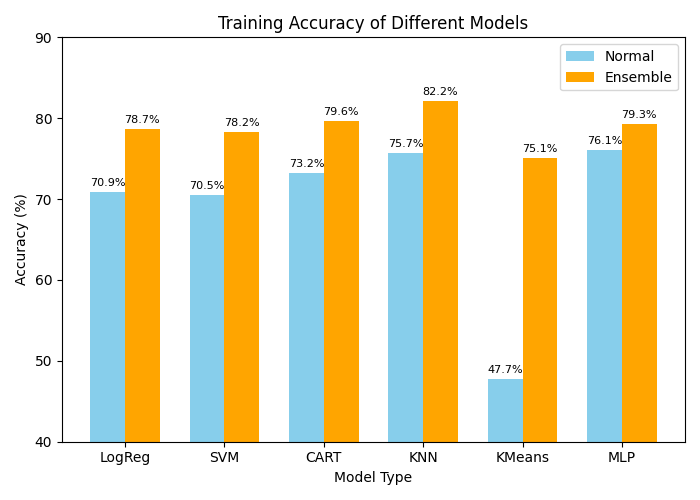
\includegraphics[width=\textwidth]{./figure/train_accs.png}
			\caption{训练集准确率}
		\end{minipage}
		\begin{minipage}{.32\textwidth}
			\centering
			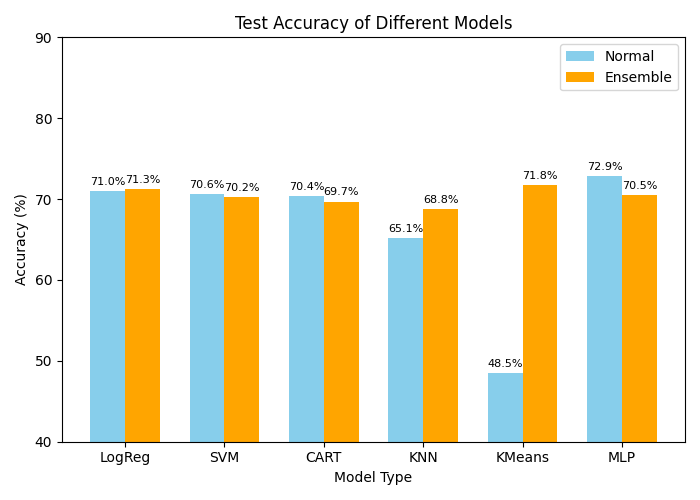
\includegraphics[width=\textwidth]{./figure/test_accs.png}
			\caption{测试集准确率}
		\end{minipage}
		\begin{minipage}{.32\textwidth}
			\centering
			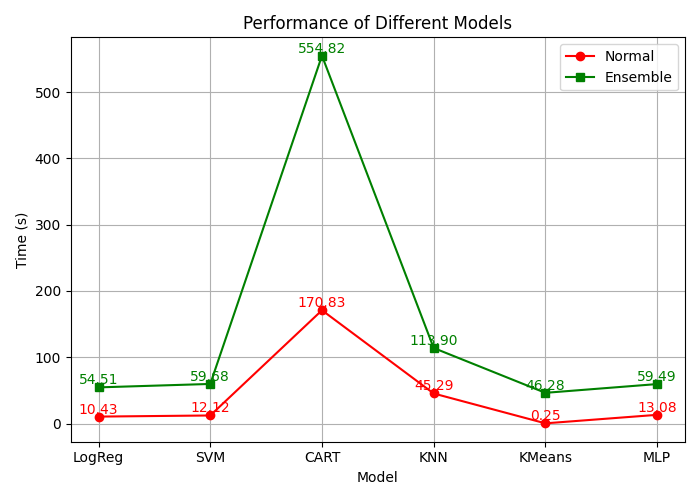
\includegraphics[width=\textwidth]{./figure/performance.png}
			\caption{不同模型的性能对比}
		\end{minipage}
	\end{figure}
	
	\subsection{集成学习对比}
	
	我们进一步对六种基础模型(逻辑斯谛回归、SVM、决策树、KNN、K-means、MLP)进行了集成,采用堆叠(Stacking)方法构建集成学习框架,以验证集成策略是否能有效提升学业困难学生识别的准确性与鲁棒性。整体结果显示,集成模型在训练集上普遍提升了性能,但在测试集上的表现则呈现一定差异化,反映出不同基础模型的泛化能力对集成效果具有显著影响。
	
	从整体精度来看,Ensemble-Kmeans 模型在测试集上取得了最高的准确率 71.75\%,显著优于其原始无监督模型 K-means(48.50\%),且测试损失也从 0.5150 降至 0.2825。这一结果表明,虽然单一 K-means 模型缺乏监督学习能力,但其生成的聚类表示在作为基学习器输入后,被更强的元学习器有效提取并加权利用,展现出良好的潜力。这种表现的提升也证明了集成学习在无监督基础上提取潜在特征的能力。
	
	Ensemble-Logistic Regression 模型在测试集上取得 71.29\% 的准确率,优于其基础模型 Logistic Regression(71.02\%),且测试损失有所下降。这表明堆叠方法可以整合多个基础模型的概率输出,从而缓解原始线性模型在复杂数据结构下的局限性。同时,该模型训练时间较为合理(54.51 秒),适合作为集成学习中的高效基线。
	
	相比之下,Ensemble-MLP 和 Ensemble-SVM 虽在训练集上表现优异(分别为 79.29\% 和 78.24\% 的训练准确率),但其在测试集上的准确率反而略有下降,分别为 70.52\% 与 70.21\%,与各自的基础模型相差不大。这种现象提示我们,深度模型与核方法本身已具较强的特征提取与拟合能力,堆叠带来的增益空间相对有限,若没有引入更加异质性的基础模型,集成效果也可能出现“边际递减”。
	
	Ensemble-KNN 的训练准确率达到 82.15\%,是所有模型中最高的,但其测试准确率为 68.83\%,未能超越其他模型。这显示出其对训练样本的极高拟合能力,但泛化能力相对较弱。由于 KNN 受邻域分布强烈影响,集成过程可能引入了冗余或局部过拟合的模式,导致整体性能受限。
	
	值得一提的是,Ensemble-Decision Tree 的测试准确率(69.70\%)略低于其基础模型(70.40\%),且损失值一致,说明在本任务中,单棵决策树模型在结构上已达到某种表达极限,集成后的增益效果并不明显。此外,其训练时间超过 550 秒,远高于其他模型,训练开销巨大,性价比较低。
	
	综合以上分析,集成学习在多数情境下能有效提升模型性能,尤其对原始性能较弱或波动较大的模型(如 K-means 和 KNN)更具稳定增益作用。然而,若基础模型已具较强表达能力或集成策略未能充分引入异质性,其提升空间有限。堆叠方法依赖多个模型输出的协同效果,因此模型间的多样性与补充性是决定集成效果的关键。在本实验场景中,选择合适的基础模型组合与高效的元模型结构,将是提升集成模型性能的下一步优化方向。
	
	\begin{figure}
		\centering
		\begin{subfigure}{.32\textwidth}
			\centering
			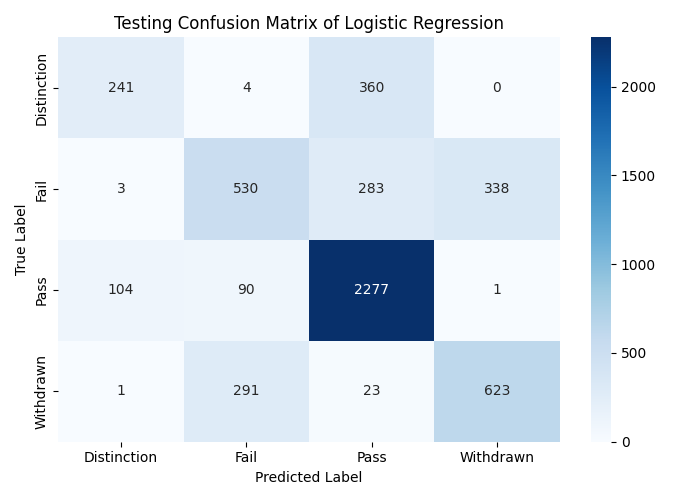
\includegraphics[width=\textwidth]{./figure/test_lr.png}
			\caption{逻辑斯谛回归}
		\end{subfigure}
		\begin{subfigure}{.32\textwidth}
			\centering
			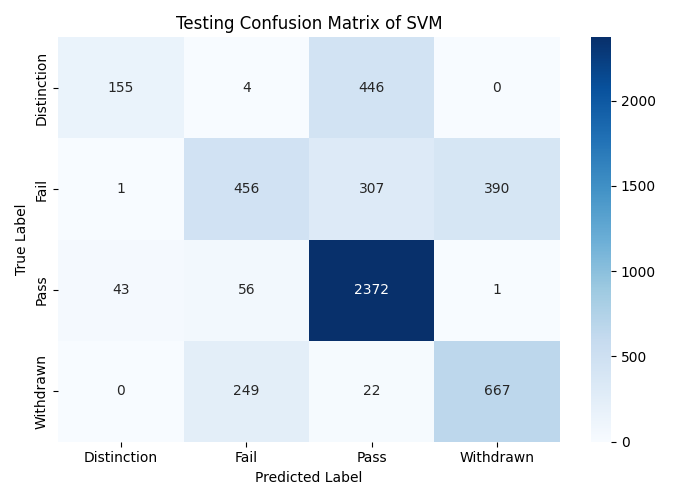
\includegraphics[width=\textwidth]{./figure/test_svm.png}
			\caption{支持向量机}
		\end{subfigure}
		\begin{subfigure}{.32\textwidth}
			\centering
			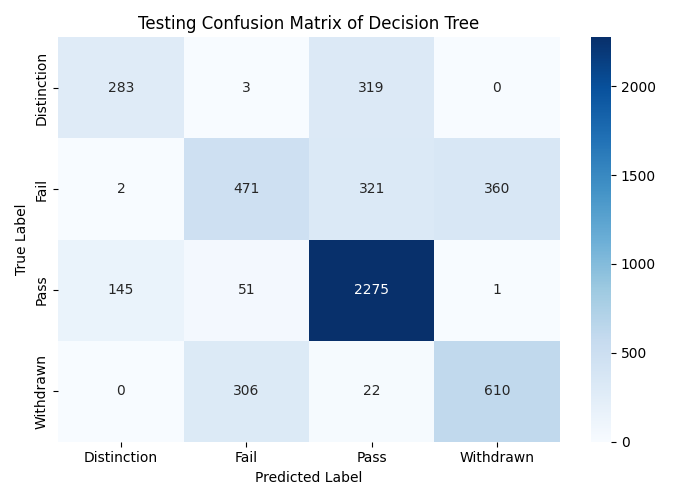
\includegraphics[width=\textwidth]{./figure/test_cart.png}
			\caption{决策树算法}
		\end{subfigure}
		
		\begin{subfigure}{.32\textwidth}
			\centering
			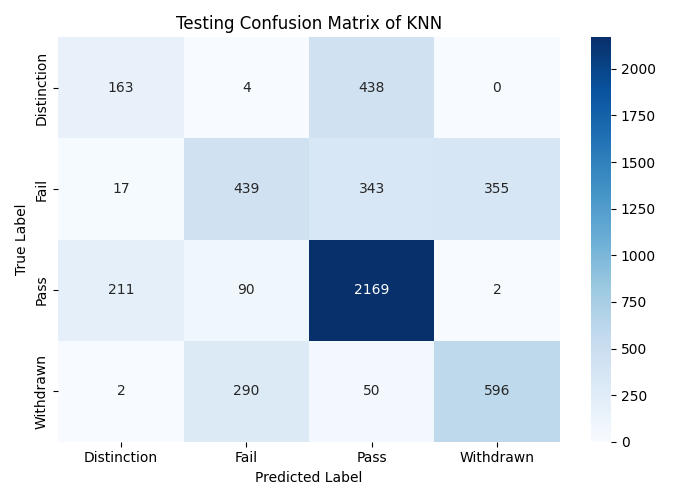
\includegraphics[width=\textwidth]{./figure/test_knn.png}
			\caption{K临近算法}
		\end{subfigure}
		\begin{subfigure}{.32\textwidth}
			\centering
			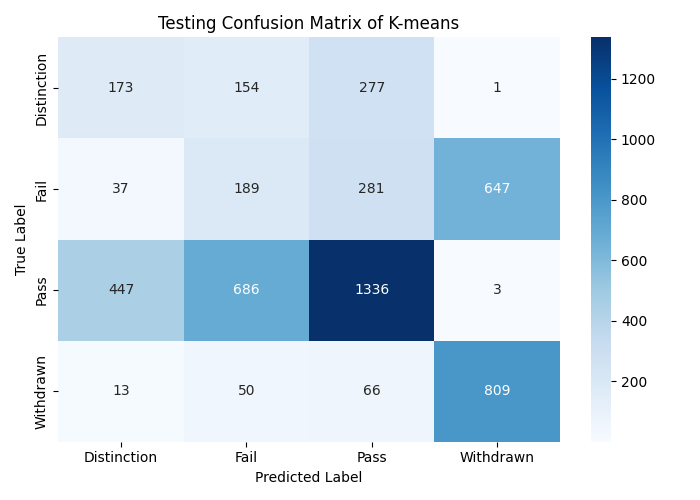
\includegraphics[width=\textwidth]{./figure/test_kmeans.png}
			\caption{K-means算法}
		\end{subfigure}
		\begin{subfigure}{.32\textwidth}
			\centering
			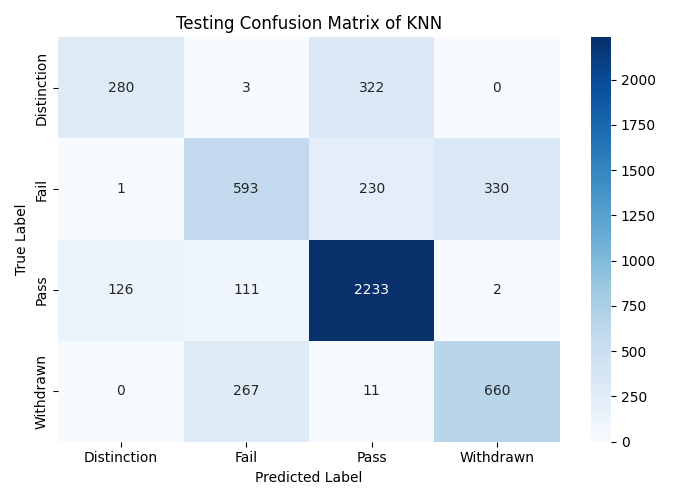
\includegraphics[width=\textwidth]{./figure/test_mlp.png}
			\caption{多层感知机}
		\end{subfigure}
		\caption{普通模型测试集混淆矩阵}
		{\small 注:多层感知机标题在进行结果导出时标题误设,此处标题应为“Test Confusion Matrix of MLP”。}
	\end{figure}
	
	\begin{figure}
		\centering
		\begin{subfigure}{.32\textwidth}
			\centering
			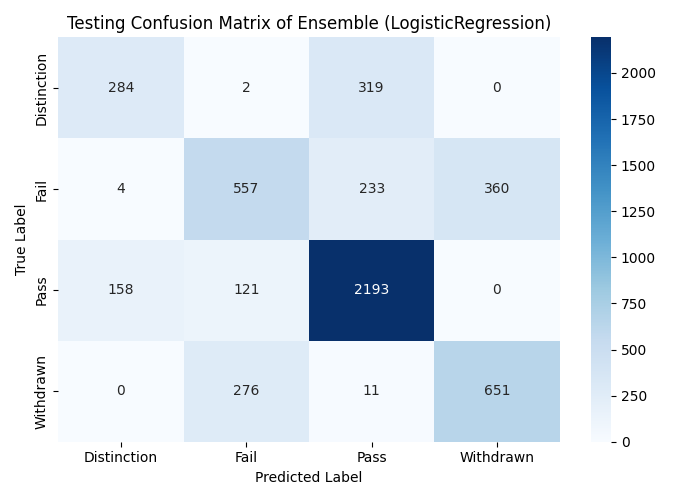
\includegraphics[width=\textwidth]{./figure/test_ensem_lr.png}
			\caption{逻辑斯谛回归}
		\end{subfigure}
		\begin{subfigure}{.32\textwidth}
			\centering
			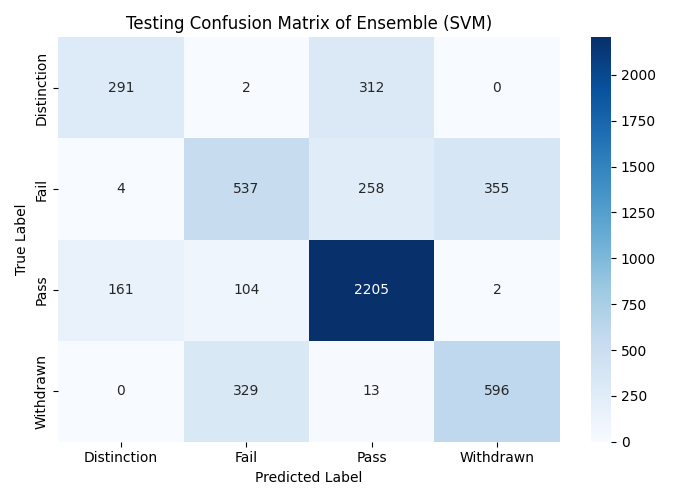
\includegraphics[width=\textwidth]{./figure/test_ensem_svm.png}
			\caption{支持向量机}
		\end{subfigure}
		\begin{subfigure}{.32\textwidth}
			\centering
			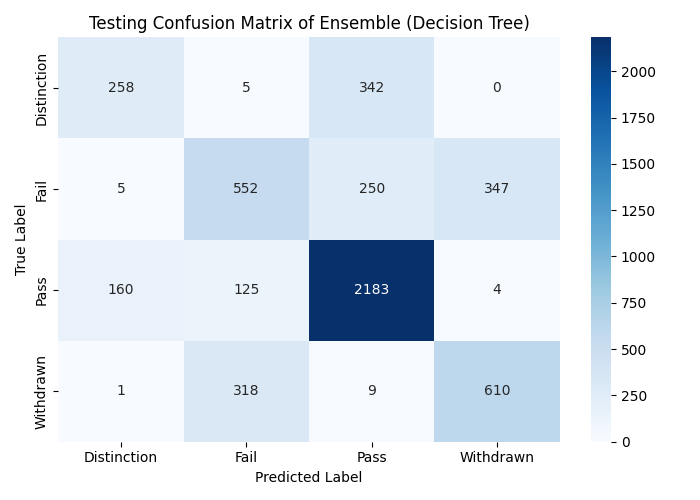
\includegraphics[width=\textwidth]{./figure/test_ensem_cart.png}
			\caption{决策树算法}
		\end{subfigure}
		
		\begin{subfigure}{.32\textwidth}
			\centering
			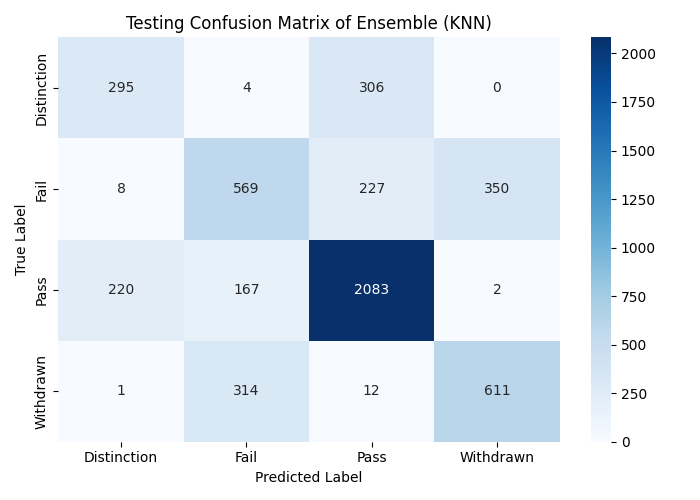
\includegraphics[width=\textwidth]{./figure/test_ensem_knn.png}
			\caption{K临近算法}
		\end{subfigure}
		\begin{subfigure}{.32\textwidth}
			\centering
			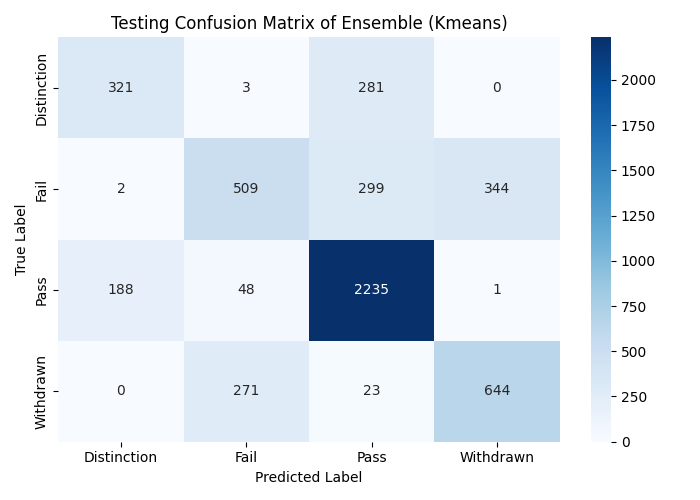
\includegraphics[width=\textwidth]{./figure/test_ensem_kmeans.png}
			\caption{K-means算法}
		\end{subfigure}
		\begin{subfigure}{.32\textwidth}
			\centering
			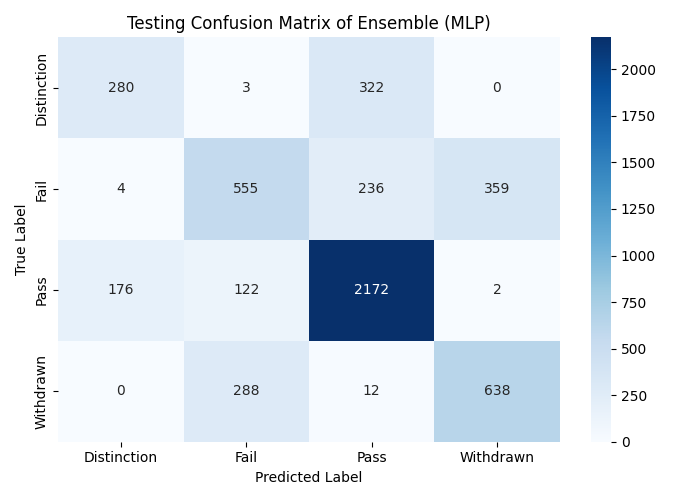
\includegraphics[width=\textwidth]{./figure/test_ensem_mlp.png}
			\caption{多层感知机}
		\end{subfigure}
		\caption{集成模型测试集混淆矩阵}
	\end{figure}
	
	\section{结论}
	
	在本次任务中,我们验证了多种判别模型与集成学习方法在“学业困难学生识别”任务中的适用性与表现差异。实验表明,不同模型在面对教育行为数据的建模能力、泛化能力和计算成本等方面各有优劣,其中具备非线性表达能力的多层感知机(MLP)展现出最强的综合性能。而集成学习策略,特别是堆叠方法,在大多数情况下能够有效整合多个模型的预测信息,从而提升整体识别效果,尤其对基础性能较弱或结构单一的模型(如 K-means、KNN)带来了明显改进。
	
	值得注意的是,集成学习的实际效果受限于基础模型的多样性与协同性。对于本身已具有较强分类能力的模型,如 MLP 和 SVM,集成后的性能提升空间相对有限,甚至可能由于信息冗余或过拟合而略微下降。因此,未来研究可进一步探索更加异质化的模型组合策略,设计更适应教育数据特性的融合机制,以提升模型的鲁棒性与少数类识别能力。
	
	总体来看,集成学习为复杂教育数据挖掘任务提供了一种有效的增强思路。在实际教育应用中,构建具有高准确性、强稳定性和可解释性的智能预警系统,不仅有助于及时发现学业风险,也为精准化教学干预与学生个性化支持提供了有力的数据支撑。未来的研究可进一步结合时序行为建模、注意力机制以及可视化解释方法,推动“学业困难学生识别”向更智能、更可信、更实用的方向发展。
	
	\let\cleardoublepage\clearpage
	
	\begin{thebibliography}{99}
		\bibitem{ref1} 谢文睿, 秦州, 贾彬彬. 机器学习公式详解[M]. 第2版. 北京:人民邮电出版社, 2023.
		\bibitem{ref2} 张伟楠, 赵寒烨, 俞勇. 动手学机器学习[M]. 第1版. 北京:人民邮电出版社, 2023.
		\bibitem{ref3} 周志华. 机器学习[M]. 第1版. 北京:清华大学出版社, 2016.
		\bibitem{ref4} Al-Azazi F A, Ghurab M. ANN-LSTM: A deep learning model for early student performance prediction in MOOC[J]. heliyon, 2023, 9(4).
		\bibitem{ref5} Baker R S, Martin T, Rossi L M. Educational data mining and learning analytics[J]. The Wiley handbook of cognition and assessment: Frameworks, methodologies, and applications, 2016: 379-396.
		\bibitem{ref6} Breiman L. Bagging predictors[J]. Machine learning, 1996, 24: 123-140.
		\bibitem{ref7} Cortes C, Vapnik V. Support-vector networks[J]. Machine learning, 1995, 20: 273-297.
		\bibitem{ref8} Cover T, Hart P. Nearest neighbor pattern classification[J]. IEEE transactions on information theory, 1967, 13(1): 21-27.
		\bibitem{ref9} Freund Y, Schapire R E. A decision-theoretic generalization of on-line learning and an application to boosting[J]. Journal of computer and system sciences, 1997, 55(1): 119-139.
		\bibitem{ref10} Gajwani J, Chakraborty P. Students’ performance prediction using feature selection and supervised machine learning algorithms[C]//International Conference on Innovative Computing and Communications: Proceedings of ICICC 2020, Volume 1. Springer Singapore, 2021: 347-354.
		\bibitem{ref11} Goodfellow I, Bengio Y, Courville A, et al. Deep learning[M]. Cambridge: MIT press, 2016.
		\bibitem{ref12} He H, Garcia E A. Learning from imbalanced data[J]. IEEE Transactions on knowledge and data engineering, 2009, 21(9): 1263-1284.
		\bibitem{ref13} Huang S, Fang N. Predicting student academic performance in an engineering dynamics course: A comparison of four types of predictive mathematical models[J]. Computers \& Education, 2013, 61: 133-145.
		\bibitem{ref14} Jayaprakash S M, Moody E W, Lauría E J M, et al. Early alert of academically at-risk students: An open source analytics initiative[J]. Journal of Learning Analytics, 2014, 1(1): 6-47.
		\bibitem{ref15} Kabra R R, Bichkar R S. Performance prediction of engineering students using decision trees[J]. International Journal of computer applications, 2011, 36(11): 8-12.
		\bibitem{ref16} Kotsiantis S B. Use of machine learning techniques for educational proposes: a decision support system for forecasting students’ grades[J]. Artificial Intelligence Review, 2012, 37: 331-344.
		\bibitem{ref17} MacQueen J. Some methods for classification and analysis of multivariate observations[C]//Proceedings of the Fifth Berkeley Symposium on Mathematical Statistics and Probability, Volume 1: Statistics. University of California press, 1967, 5: 281-298.
		\bibitem{ref18} Mohamad S K, Tasir Z. Educational data mining: A review[J]. Procedia-Social and Behavioral Sciences, 2013, 97: 320-324.
		\bibitem{ref19} Nghe N T, Janecek P, Haddawy P. A comparative analysis of techniques for predicting academic performance[C]//2007 37th annual frontiers in education conference-global engineering: knowledge without borders, opportunities without passports. IEEE, 2007: T2G-7-T2G-12.
		\bibitem{ref20} Papamitsiou Z, Economides A A. Learning analytics and educational data mining in practice: A systematic literature review of empirical evidence[J]. Journal of Educational Technology \& Society, 2014, 17(4): 49-64.
		\bibitem{ref21} Pardos Z A, Heffernan N T. Modeling individualization in a bayesian networks implementation of knowledge tracing[C]//User Modeling, Adaptation, and Personalization: 18th International Conference, UMAP 2010, Big Island, HI, USA, June 20-24, 2010. Proceedings 18. Springer Berlin Heidelberg, 2010: 255-266.
		\bibitem{ref22} Piech C, Bassen J, Huang J, et al. Deep knowledge tracing[J]. Advances in neural information processing systems, 2015, 28.
		\bibitem{ref23} Quinlan J R. Induction of decision trees[J]. Machine learning, 1986, 1: 81-106.
		\bibitem{ref24} Soni A, Kumar V, Kaur R, et al. Predicting student performance using data mining techniques[J]. International Journal of Pure and Applied Mathematics, 2018, 119(12): 221-227.
		\bibitem{ref25} Wolpert D H. Stacked generalization[J]. Neural networks, 1992, 5(2): 241-259.
		\bibitem{ref26} Zhang L, Rangwala H. Early identification of at-risk students using iterative logistic regression[C]//Artificial Intelligence in Education: 19th International Conference, AIED 2018, London, UK, June 27–30, 2018, Proceedings, Part I 19. Springer International Publishing, 2018: 613-626.
	\end{thebibliography}
	
\end{document}
